\chapter{Wprowadzenie}\label{ch:wprowadzenie}

\begin{sekcja}{Cel dokumentu}
Ten dokument opisuje, jak przygotować i wykonać misję balonu stratosferycznego na platformie Stardust NEXT. Platforma to mały balon lateksowy z gondolą z pudełek styropianowych i odcinaczem mechanicznym.

Dokument daje niezbędne minimum, aby nowy zespół wyjął sprzęt z szafki i wykonał misję. Dokument jest ogólny: działa dla każdej przyszłej misji. Dane konkretnych misji są tylko w rozdziale~\ref{ch:historia} i w wypełnionych formularzach.

Dokument zawiera:
\begin{itemize}
  \item historię platformy i wnioski z poprzednich lotów,
  \item planowanie misji: od celu i ładunku do decyzji o starcie,
  \item wymagania prawne,
  \item segment naziemny: stanowisko startowe, tankowanie, stacje odbiorcze,
  \item segment lotny: powłoka, spadochron, olinowanie, odcinacz, gondola,
  \item elektronikę i łączność radiową,
  \item oprogramowanie do predykcji i śledzenia,
  \item instrukcje montażu i wykaz materiałów,
  \item zasady prowadzenia projektu i dokumentacji,
  \item formularze do druku i notatki terenowe.
\end{itemize}
\end{sekcja}

\begin{sekcja}{Jak używać tego dokumentu}
\begin{enumerate}
  \item Przeczytaj rozdział~\ref{ch:historia} „\nameref{ch:historia}”. Wnioski z poprzednich lotów wyjaśniają, dlaczego procedury wyglądają tak, jak wyglądają.
  \item Zacznij planowanie od rozdziału~\ref{ch:planowanie} „\nameref{ch:planowanie}”, co najmniej 3--4 miesiące przed planowanym lotem.
  \item Sprawdź sprzęt z szafki według rozdziału~\ref{ch:materialy} „\nameref{ch:materialy}”.
  \item Wydrukuj formularze z dodatku~\ref{dod:formularze}. Wypełniaj je długopisem w trakcie przygotowań i w dniu startu.
  \item Po misji przenieś notatki terenowe i wnioski do repozytorium dokumentacji.
\end{enumerate}

W tekście są dwa rodzaje ramek:

\begin{uwaga}Informacja o zagrożeniu dla ludzi, sprzętu albo powodzenia misji.\end{uwaga}

\begin{wskazowka}Praktyczna rada z poprzednich misji.\end{wskazowka}
\end{sekcja}

\begin{sekcja}{Najpierw bezpieczeństwo i rozsądek}
Ten dokument jest wzorem, nie przepisem. Procedury i dokumentacja są ważne, ale najważniejsze jest to, aby misja przebiegła bezpiecznie i aby wszyscy dobrze się bawili.

\begin{itemize}
  \item Nie stresuj się, że pominiesz jakiś krok, jeżeli możesz się upewnić, że mimo to wszystko będzie bezpieczne. Rozsądek przede wszystkim.
  \item Dopasuj procedury do swojej misji. Gdy coś nie pasuje -- zmień to i zapisz dlaczego.
  \item Balon stratosferyczny to jeden z najprostszych sposobów, aby zdobyć praktyczne doświadczenie w całym przekroju projektu: od celu naukowego, przez budowę i testy, formalności i logistykę, do analizy wyników.
  \item Publikuj wyniki na konferencjach -- w szczególności na sympozjum ESA PAC (\emph{ESA Symposium on European Rocket and Balloon Programmes and Related Research}). Inne miejsca dla studenckich projektów balonowych: konferencja AHAC i czasopismo \emph{Journal of High Altitude Ballooning}~\cite{sba}. Czytaj artykuły naukowe z tych i innych konferencji.
\end{itemize}

\begin{center}\sffamily\large\color{sdorange} Stay curious, have fun.\end{center}
\end{sekcja}

\begin{sekcja}{Platforma Stardust NEXT}
Platforma Stardust NEXT to zestaw sprzętu i procedur do lotów balonów stratosferycznych. Koło Naukowe SimLE (Politechnika Gdańska) opracowało platformę na podstawie doświadczeń z projektu Stardust~\cite{iac2023,pac2024}.

Platforma ma trzy zadania:
\begin{enumerate}
  \item Wynieść ładunek badawczy do stratosfery i bezpiecznie sprowadzić go na ziemię.
  \item Oddzielić elektronikę platformy od ładunku. Zespół platformy i zespół badawczy pracują niezależnie. Ładunek musi tylko zmieścić się w standardowym pudełku i w limicie masy.
  \item Używać powtarzalnych komponentów i procedur, aby każdy nowy skład zespołu mógł wykonać misję.
\end{enumerate}

\dwafoto{2023_zestaw_przed_startem}{Zestaw lotny przed startem: gondola gotowa, olinowanie rozłożone, w tle tankowanie powłoki (26.05.2023).}
{2023_balon_po_tankowaniu}{Powłoka po tankowaniu, przytrzymywana folią przed startem (26.05.2023).}
\end{sekcja}

\begin{sekcja}{Typowy lot}
Typowy lot balonu lateksowego trwa około 2,5--3 godzin (rysunek~\ref{fig:profil-typowy}):
\begin{enumerate}
  \item Wznoszenie z prędkością około \SI{5}{m/s}.
  \item Pęknięcie powłoki na wysokości około 28--35~km albo odcięcie ładunku przez odcinacz.
  \item Opadanie na spadochronie. Wysoko spadochron opada bardzo szybko, bo powietrze jest rzadkie. Przy ziemi prędkość spada do około \SI{5}{m/s}.
  \item Lądowanie w odległości od kilkunastu do ponad 100~km od miejsca startu. Odległość zależy od wiatru.
\end{enumerate}

\begin{center}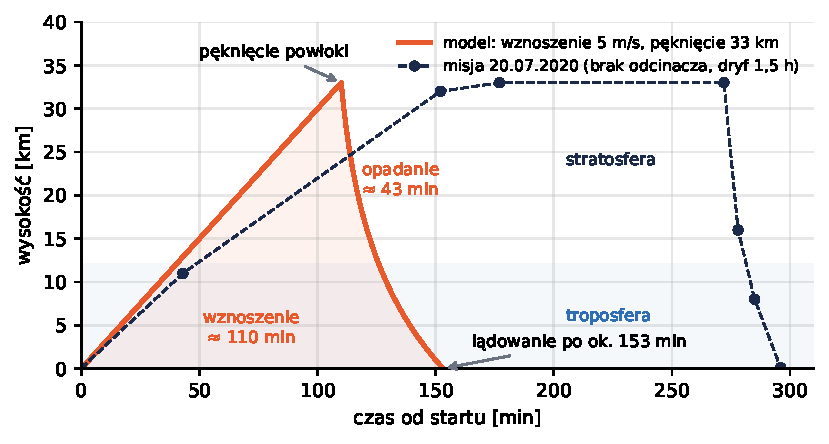
\includegraphics[width=\linewidth]{profil_typowy}\end{center}
\captionof{figure}{Typowy lot: model (wznoszenie \SI{5}{m/s}, pęknięcie na \SI{33}{km}) i dane misji z 20.07.2020. W 2020 roku balon nie pękł na przewidywanej wysokości i dryfował prawie 2~h na \SI{33}{km}, bo nie miał odcinacza~\cite{raport2020}.}\label{fig:profil-typowy}
\end{sekcja}

\begin{sekcja}{Warunki w stratosferze}
Stratosfera to warstwa atmosfery od około 12--15 do \SI{50}{km}. Warunki w stratosferze:
\begin{itemize}
  \item temperatura powietrza do około \SI{-60}{\degreeCelsius},
  \item ciśnienie poniżej \SI{100}{hPa}; na wysokości \SI{33}{km} około \SI{7}{hPa} -- to prawie próżnia,
  \item silne promieniowanie UV i kosmiczne,
  \item bardzo słaba wymiana ciepła z powietrzem: elektronika nie oddaje ciepła przez konwekcję i może się przegrzać mimo mrozu (rozdział~\ref{ch:elektronika}).
\end{itemize}
\foto[0.85\linewidth]{2020_kamera_pokladowa_stratosfera}{Widok z kamery pokładowej 360° w troposferze (20.07.2020). Zakrzywienie horyzontu to efekt obiektywu typu rybie oko. Bateria kamery wyczerpała się po około 30 minutach lotu~\cite{raport2020}.}
\end{sekcja}

\begin{sekcja}{Architektura misji}
Misja ma dwa segmenty.

\begin{minipage}[t]{0.47\linewidth}
\textbf{Segment naziemny} (rozdział~\ref{ch:naziemny}):
\begin{itemize}
  \item stanowisko startowe,
  \item zestaw do tankowania,
  \item stacja odbiorcza stacjonarna,
  \item stacja odbiorcza mobilna w samochodzie pościgowym,
  \item oprogramowanie do planowania, predykcji i śledzenia.
\end{itemize}
\end{minipage}\hfill
\begin{minipage}[t]{0.47\linewidth}
\textbf{Segment lotny} (rozdział~\ref{ch:lotny}), od góry:
\begin{enumerate}
  \item powłoka z helem,
  \item krętlik,
  \item spadochron,
  \item olinowanie z odcinaczem,
  \item gondola platformy,
  \item gondola ładunku.
\end{enumerate}
\end{minipage}
\end{sekcja}

\begin{sekcja}{Fazy misji}
Misja to zwieńczenie kilku miesięcy przygotowań. Sam lot trwa kilka godzin. Nazwy faz odpowiadają typowym fazom projektu (inicjacja, planowanie, realizacja, zamknięcie) i kampanii startowej programów takich jak BEXUS.

\renewcommand{\arraystretch}{1.35}
\begin{tabularx}{\linewidth}{@{}P{30mm}LP{36mm}@{}}
\toprule
\textbf{Faza} & \textbf{Zadania} & \textbf{Rozdział / formularz}\\\midrule
Inicjacja & Cel misji, wymagania ładunku, projekt i budowa eksperymentu. & \ref{ch:planowanie}, F2\\
Planowanie lotu & Bilans masy, ilość gazu, predykcja trajektorii, wybór terminów i miejsc. & \ref{ch:planowanie}, F4\\
Formalności & Klasa balonu, zgłoszenie do PAŻP, ubezpieczenie, licencja radiowa. & \ref{ch:prawo}, F3\\
Budowa i testy & Montaż, testy w zimnie, zasięgu, odcinacza, czasu pracy. & \ref{ch:montaz}, F5\\
Przegląd gotowości & Przegląd gotowości do startu: decyzja „leci / nie leci”. & \ref{ch:planowanie}, F6\\
Start & Kampania startowa: stanowisko, tankowanie, start. & \ref{ch:naziemny}, F9--F11\\
Lot i pościg & Odbiór telemetrii, jazda w kierunku predykcji. & \ref{ch:oprogramowanie}, F12\\
Odzyskanie & Lokalizacja ładunku, zabezpieczenie danych. & F13\\
Analiza i zamknięcie & Raport, wnioski, aktualizacja dokumentacji. & \ref{ch:projekt}, F14\\
\bottomrule
\end{tabularx}
\end{sekcja}
